\chapter{Krav}
Ud fra projektformuleringen er der formuleret en række krav til projektet. Disse indebærer to use cases og et antal ikke-funktionelle krav. 

På figur \ref{fig:useCaseDiagram} ses Use Case diagrammet for systemet.

\begin{figure}[H]
	\centering
	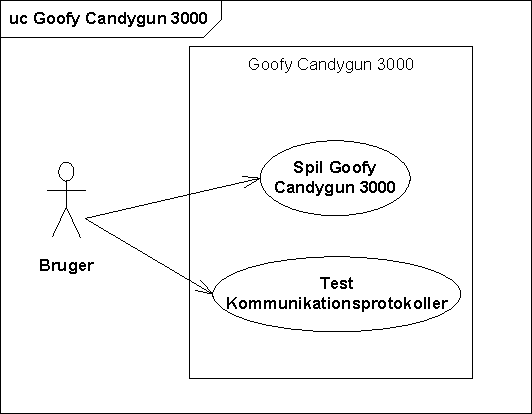
\includegraphics[width=0.80\textwidth]{Kravsspecifikation/images/usecaseDiagram.png}
	\caption{Use case diagram}
	\label{fig:useCaseDiagram}
\end{figure}

\section{Aktørbeskrivelse}
På figur \ref{fig:useCaseDiagram} ses det at der er én primær bruger for systemet, brugeren. Denne beskrives her.

\subsection{Aktør - Bruger}

\begin{tabularx}{\textwidth}{| p{2cm} | p{9.1cm} |}
	\hline
	Aktørens Navn: & Bruger \\ 
	\hline
	Alternativ Navn: & Spiller \\
	\hline
	Type: & Primær \\
	\hline
	Beskrivelse: & Brugeren initierer Goofy Candy Gun, ved at vælge spiltype på brugergrænsefladen. Derudover har brugeren mulighed for at stoppe spillet igennem brugergrænsefladen. Brugeren vil under spillet interagere med Goofy Candy Gun gennem Wii-Nunchucken. \newline
	Brugeren starter også Goofy Candy Gun system-testen for at verificere om det er operationelt. \\
	\hline
\end{tabularx}

\newpage
\section{Use case beskrivelse}
\subsection{Use case 1}
Denne Use Case indebærer at spille Goofy Candygun 3000, og den initieres af brugeren. Det første der sker i use case er, at brugeren skal vælge, hvilken type spil han/hun gerne vil spille. Det betyder, at det skal bestemmes, om det skal være et enpersonsspil, topersonersspil eller om det skal være party mode. Herefter skal der vælges, hvor mange skud et spil skal vare og disse skal puttes i magasinet. Når dette er gjort kan spillet gå i gang. Brugeren indstiller kanonen med Wii-nunchuck og affyrer den. Herefter lader systemet et nyt skud og samme procedure gentages. Til slut vises information om spillet på brugergrænsefladen, brugeren afslutter spillet ved at trykke på knappen på brugergrænsefladen og denne vender tilbage til starttilstanden. \textbf{\#ref} til fully dressed use case 1.

\subsection{Use case 2}
Denne Use Case skal bruges til at teste systemets kommunikationsprotokoller, altså om der er forbindelse mellem alle hardwareblokke forbundet via systemets busser, og om disse kan fortolke kommandoer korrekt. Hvis der bliver fundet fejl, raporteres disse til brugeren via brugergrænsefladen. Use Casen initieres af brugeren, hvor der herefter bliver sendt informationer ud til de forskellige dele af systemet, som så gerne skal sende svar tilbage igen. Hvis det sker for alle dele, vil brugergrænsefladen til sidst meddele, at use casen er gennemført. \textbf{\#ref} til fully dressed use case 2.


\section{Ikke-funktionelle krav}
De ikke-funktionelle krav siger noget om, hvordan systemet skal bygges, og hvilke specifikationer det skal have. I dette tilfælde er der udarbejdet syv krav, hvor der er et der siger noget om, hvordan kanonen skal kunne drejes. Nogle siger noget om kanonens størrelse, hvor der også er specificeret, hvor stort projektilet den skal affyre må være og et siger, hvor langt den skal kunne skyde. Der er et, der siger, hvor lang tid det må tage at skyde et projektil afsted og hvor hurtig den skal være til at lade kanonen igen. Endelig er der et, der specificerer, hvordan den grafiske brugergrænseflade skal se ud. Deciderede værdier for de enkelte krav kan læses i bilag. \textbf{\#ref}







